\documentclass{dependencies/acm_proc_article-sp}

\usepackage{url}
\usepackage{color}
\usepackage{verbatim}
\usepackage{listings}
\lstset{
  language=C++,             % choose the language of the code
  basicstyle=\small,       % the size of the fonts that are used for the code
  numbers=left,                   % where to put the line-numbers
  numberstyle=\footnotesize,      % the size of the fonts that are used for the line-numbers
  stepnumber=0,                   % the step between two line-numbers. If it is 1 each line will be numbered
  numbersep=5pt,                  % how far the line-numbers are from the code
  backgroundcolor=\color{white},  % choose the background color. You must add \usepackage{color}
  showspaces=false,               % show spaces adding particular underscores
  showstringspaces=false,         % underline spaces within strings
  showtabs=false,                 % show tabs within strings adding particular underscores
  %frame=single,                   % adds a frame around the code
  tabsize=2,              % sets default tabsize to 2 spaces
  captionpos=t,                   % sets the caption-position to bottom
  breaklines=false,        % sets automatic line breaking
  breakatwhitespace=false,    % sets if automatic breaks should only happen at whitespace
  escapeinside={\%}{)}          % if you want to add a comment within your code
}

% Get rid of the permission block
\makeatletter
\let\@copyrightspace\relax
\makeatother

\begin{document}

%\title{ Distributed Systems: Project Description }
\title{ Distrivia: A Distributed Trivia Game }
\numberofauthors{3}
\author{
\alignauthor
Brian Gianforcaro \\
       \affaddr{Rochester Institute of Technology}\\
       \email{bjg1955@rit.edu}
\alignauthor
Steven Glazer \\
       \affaddr{Rochester Institute of Technology}\\
       \email{sfg6126@rit.edu}
\alignauthor
Samuel Milton \\
       \affaddr{Rochester Institute of Technology}\\
       \email{srm2997@rit.edu}
}
\maketitle

%\begin{abstract}
%In this paper we detail our current progress on our distributed trivia game.
%We will explain what has been done so far, what we need to do, and how we
%have met the requirements for the project. We also discuss the architecture
%for our system.
%\end{abstract}

\section{Project Motivation}
\section{Architecture}
\begin{figure}[h!]
  \centering
    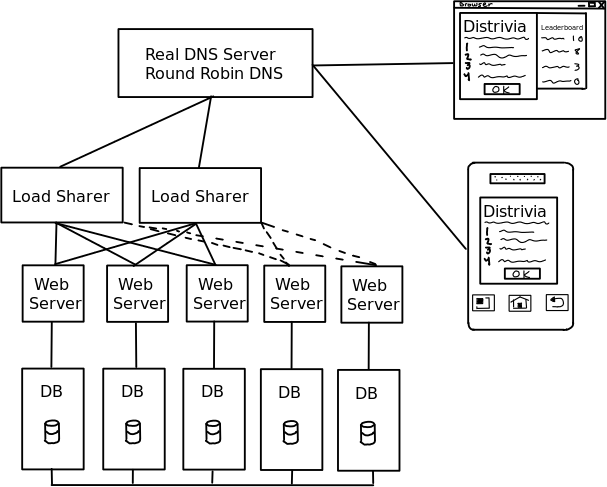
\includegraphics[scale=0.4]{diagram.png}
   \caption{High level overview of the system}
 \end{figure}

\subsection {Servers}
Currently, we have 6 servers running on Amazon's Elastic Compute Cloud \cite{aec}. One server is being used as a web-monitor
host running Monit\cite{monit}. We are able to login to the web-monitor to see the status of all our
servers, databases, and load sharers. This will help us manage whether or not the services
are running and allow us to track down any problems, if they arise. Three
servers are all running our server application and hosting the databases.
We also have two final servers that we have setup as hot spares in the event
of partial or total failure.
Each server contains the server application that responds to clients as well as
the Riak \cite{riak} databases. Riak auto-synchronizes the databases between the 5 servers.
Note that the hot spares are setup to be part of the database cluster so they
have a full copy of the database on hand, however they don't accept any reads
or writes directly. This allows for them to immediately be ready for read/writes in the event that the original servers are down.
With this configuration if we were to add a server, we would just need to update 
Riak and it would sync the databases to any additional servers as well. These servers,
therefore, all contain the same information. If any servers go down, the distributed
system would still run fine. We could have all servers go down except one and still
be reliably handling requests.

\subsection{Server Applications}
The server is currently almost feature complete, but still needs a lot of
testing. Client registration, and login are all supported. A client can
join a game, retrieve questions for that game, and answer questions. Both a
global leader board and individual per game leader board can also be requested.
We recently refactored our API to be more universally consistent.
The servers and clients now work on a more consistent basis where the clients all expect the same information and use the same calls.

\subsection{Traffic}
We have two load sharers set up. Both sharers are currently configured to
divide the requests among the three active servers and, if need be, the two hot spares. The duplicate sharers allow
for a load distributer to go down and we would still be able to serve requests
to the servers. These load sharers are selected by the clients using round
robin DNS where distrivia.lame.ws will select either load distributer that is
up at random. If a load distributer should go down or become unreachable the
DNS service will no longer serve that hosts DNS record until it is again
reachable. This provides us with stability for accessing the servers. The
load sharers are set up to attempt to connect to a server twice in a one second
period before deeming it dead and removing it from its list of servers to direct clients towards.
Currently we are using the NGINX \cite{nginx} in a reverse proxy configuration
for our load sharing needs.

\subsection{Clients}
Our focus for clients has been on a web-based client and an Android application.
Both clients have most of the workings completed. The web-based client will
be run from desktop platforms and laptop platforms. The Android client will run
on any Android phone running OS 2.1 or higher and does not use any unique services that require specific
hardware. Both clients are nearly fully-functional. They can, currently, login/register
players, view leaderboards, join public games, and compete in public games. We are actively adding features to both clients, daily.
We have also started development on an iPhone application for distrivia. This client does not yet communicate with the server, but 
it does implement nearly all the views seen in the other clients. We have been setting up the network communication for the iPhone
platform as well.

\subsection{Messages}
We are currently using the https protocol for our messages. This provides a secure
and usable messaging system that we have designed our client and server APIs to use.
The actual messages are sent and received in two way's. Initially a user session key is
generated using the UUID\cite{uuid} algorithm and returned to the user on successful
authentication. This session key is then passed back to the server with every in coming
message. Messages are sent to the server using POST and GET request methods supported
by the HTTP protocol. Responses from the server are in the form of JSON \cite{json} objects.
JSON is a small, easily parseable format, representing objects in a human readable format as
they would be represented in JavaScript. With the web client the JSON object returned from
the server is instantly usable, however for the Android client we have to parse the JSON object
into a native Java object. The Android SDK provides libraries to do this, located in the
org.json \cite{orgjson} package name space.

\section{Design}

\section{Implementation}

\section{Lessons Learned}

\section{Future Work}

\newpage
%
% The following two commands are all you need in the
% initial runs of your .tex file to
% produce the bibliography for the citations in your paper.
\bibliographystyle{abbrv}
\bibliography{bibliography}  % sigproc.bib is the name of the Bibliography in this case
% You must have a proper ".bib" file
%  and remember to run:
% latex bibtex latex
% to resolve all references
%
% ACM needs 'a single self-contained file'!
%
%APPENDICES are optional
\balancecolumns
% That's all folks!
\end{document}
